% move all configuration stuff into one file so we can focus on the content
\documentclass[aspectratio=169,hyperref={pdfpagelabels=false,colorlinks=true,linkcolor=white,urlcolor=lightblue},xcolor={table},t]{beamer}

%%%%%%%%%%%%%%%%%%%%%%%%%%%%%%%%%%%%%%%%%%%%%%%%%%%%%%%%%%%%%%%%%%%%%%%%%%%%%%%%%%
%%%%%%%%%%%%%%%%%%%%%%%%%%%%%%%%%%%%%%%%%%%%%%%%%%%%%%%%%%%%%%%%%%%%%%%%%%%%%%%%%%
% packages
\usepackage{pict2e}
\usepackage{epic}
\usepackage{amsmath,amsfonts,amssymb}
\usepackage{units}
\usepackage{fancybox}
\usepackage[absolute,overlay]{textpos} 
%\usepackage[table]{xcolor}
\usepackage{animate}
\usepackage{gensymb}
%\usepackage{graphicx}
%\usepackage{longtable}
\usepackage{multirow}
\usepackage{silence}
\usepackage{tikz}
\usepackage[backend=bibtex,style=ieee]{biblatex}
\AtEveryCitekey{\iffootnote{\tiny}{}}
%\addbibresource{include/references}



% fontsize
\let\Tiny=\tiny

%%%%%%%%%%%%%%%%%%%%%%%%%%%%%%%%%%%%%%%%%%%%%%%%%%%%%%%%%%%%%%%%%%%%%%%%%%%%%%%%%%
%%%%%%%%%%%%%%%%%%%%%%%%%%%%%%%%%%%%%%%%%%%%%%%%%%%%%%%%%%%%%%%%%%%%%%%%%%%%%%%%%%
% warnings
\pdfsuppresswarningpagegroup=1
\WarningFilter{biblatex}{Patching footnotes failed}
\WarningFilter{latexfont}{Font shape}
\WarningFilter{latexfont}{Some font shapes}
\WarningFilter{gensymb}{Not defining}


%%%%%%%%%%%%%%%%%%%%%%%%%%%%%%%%%%%%%%%%%%%%%%%%%%%%%%%%%%%%%%%%%%%%%%%%%%%%%%%%%%
%%%%%%%%%%%%%%%%%%%%%%%%%%%%%%%%%%%%%%%%%%%%%%%%%%%%%%%%%%%%%%%%%%%%%%%%%%%%%%%%%%
% theme & layout
\usetheme{Frankfurt}
\useinnertheme{rectangles}


%%%%%%%%%%%%%%%%%%%%%%%%%%%%%%%%%%%%%%%%%%%%%%%%%%%%%%%%%%%%%%%%%%%%%%%%%%%%%%%%%%
\setbeamertemplate{frametitle}[default][colsep=-4bp,rounded=false,shadow=false]
\setbeamertemplate{frametitle}
{%
    \nointerlineskip%
    %\vskip-0.5ex
    \begin{beamercolorbox}[wd=\paperwidth,ht=3.5ex,dp=0.6ex]{frametitle}
        \hspace*{1.3ex}\insertframetitle%
        
        \hspace*{1.3ex}\small\insertframesubtitle%
    \end{beamercolorbox}%
    \begin{textblock*}{100mm}(13.75cm,1cm)
        
\includegraphics[height=.4cm,keepaspectratio]{../shared/Logo_GTCMT_white}
    \end{textblock*}
}


%%%%%%%%%%%%%%%%%%%%%%%%%%%%%%%%%%%%%%%%%%%%%%%%%%%%%%%%%%%%%%%%%%%%%%%%%%%%%%%%%%
\setbeamertemplate{title page}[default][colsep=-4bp,rounded=false,shadow=false]
\setbeamertemplate{title page}
{
    %\begin{textblock*}{100mm}(15cm,.51cm)
            %\href{https://github.com/alexanderlerch/ACA-Slides/blob/2nd_edition/\jobname.pdf}{\includegraphics[height=.5cm,keepaspectratio]{graph/Logo_github}}\hspace*{2ex}
    %\end{textblock*}
    %\begin{textblock*}{100mm}(15cm,1.3cm)
            %\href{\IEEELink}{\includegraphics[height=.5cm,keepaspectratio]{graph/icon/book}}\hspace*{2ex}
    %\end{textblock*}
    \vskip-10ex
    \begin{beamercolorbox}[wd=\paperwidth,ht=.7\paperheight,dp=0.6ex]{frametitle} %35ex
        %\begin{flushright}
            %\href{http://www.gtcmt.gatech.edu}{
\includegraphics[height=.8cm,keepaspectratio]{graph/Logo_GTCMT_black}}\hspace*{2ex}
        %\end{flushright}
        
        \hspace*{1.8ex}\LARGE\inserttitle%
        
        \vspace*{.5ex}
        
        \hspace*{1.3ex}\small\insertsubtitle%
        
        \vspace*{.5ex}
    \end{beamercolorbox}%
    \nointerlineskip%
    \begin{beamercolorbox}[wd=\paperwidth,ht=.4\paperheight,dp=0.6ex]{page number in head/foot}
        %\vspace*{-.5ex}
        \hspace*{1.7ex}\small\insertauthor%
        
        %\hspace*{1.7ex}\small }%
        
        \vspace*{12ex}
        \vfill
        \begin{flushright}
            \href{http://www.gtcmt.gatech.edu}{
\includegraphics[height=.5cm,keepaspectratio]{../shared/Logo_GTCMT_black}}\hspace*{2ex}
        \end{flushright}
    \end{beamercolorbox}%
}


%%%%%%%%%%%%%%%%%%%%%%%%%%%%%%%%%%%%%%%%%%%%%%%%%%%%%%%%%%%%%%%%%%%%%%%%%%%%%%%%%%
%\makeatother
\setbeamertemplate{footline}
{
  \leavevmode%
  \hbox{%
  \begin{beamercolorbox}[wd=.5\paperwidth,ht=2.25ex,dp=1ex,left,leftskip=1ex]{page number in head/foot}%
    \insertsubtitle
  \end{beamercolorbox}%
  \begin{beamercolorbox}[wd=.5\paperwidth,ht=2.25ex,dp=1ex,right,rightskip=1ex]{page number in head/foot}%
    \hfill
    \insertframenumber{} / \inserttotalframenumber
  \end{beamercolorbox}}%
  \vskip0pt%
}
%\makeatletter


%%%%%%%%%%%%%%%%%%%%%%%%%%%%%%%%%%%%%%%%%%%%%%%%%%%%%%%%%%%%%%%%%%%%%%%%%%%%%%%%%%
\beamertemplatenavigationsymbolsempty
\setbeamertemplate{navigation symbols}{}
\setbeamertemplate{blocks}[default]%[rounded=false,shadow=false]
\setbeamertemplate{itemize item}[square]
\setbeamertemplate{itemize subitem}[circle]
\setbeamertemplate{itemize subsubitem}[triangle]
\setbeamertemplate{enumerate item}[square]
\setbeamertemplate{enumerate subitem}[circle]
\setbeamertemplate{enumerate subsubitem}[circle]


%%%%%%%%%%%%%%%%%%%%%%%%%%%%%%%%%%%%%%%%%%%%%%%%%%%%%%%%%%%%%%%%%%%%%%%%%%%%%%%%%%
% colors
\setbeamercolor{structure}{fg=darkgray}
\setbeamercovered{transparent} %invisible
\setbeamercolor{bibliography entry author}{fg=black}
\setbeamercolor*{bibliography entry title}{fg=black}
\setbeamercolor*{bibliography entry note}{fg=black}
\setbeamercolor{frametitle}{fg=black}
\setbeamercolor{title}{fg=white}
\setbeamercolor{subtitle}{fg=white}
\setbeamercolor{frametitle}{fg=white}
\setbeamercolor{framesubtitle}{fg=white}
\setbeamercolor{mini frame}{fg=white, bg=black}
\setbeamercolor{section in head/foot}{fg=white, bg=darkgray}
\setbeamercolor{page number in head/foot}{fg=black, bg=gtgold}
\setbeamercolor{item projected}{fg=white, bg=black}

%---------------------------------------------------------------------------------

%%%%%%%%%%%%%%%%%%%%%%%%%%%%%%%%%%%%%%%%%%%%%%%%%%%%%%%%%%%%%%%%%%%%%%%%%%%%%%%%%%
%%%%%%%%%%%%%%%%%%%%%%%%%%%%%%%%%%%%%%%%%%%%%%%%%%%%%%%%%%%%%%%%%%%%%%%%%%%%%%%%%%
% title information
\title[]{MUSI6202: Digital Signal Processing for Music}   
\author[alexander lerch]{alexander lerch} 
%\institute{~}
%\date[Alexander Lerch]{}
%\titlegraphic{\vspace{-16mm}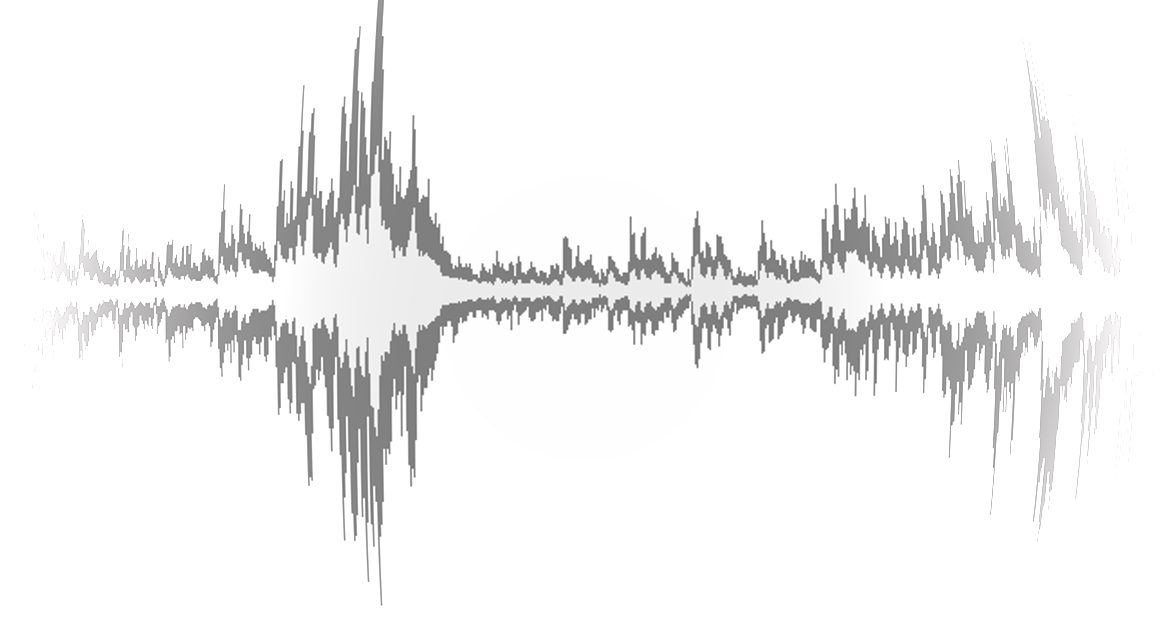
\includegraphics[width=\textwidth,height=3cm]{title}}

%%%%%%%%%%%%%%%%%%%%%%%%%%%%%%%%%%%%%%%%%%%%%%%%%%%%%%%%%%%%%%%%%%%%%%%%%%%%%%%%%%
%%%%%%%%%%%%%%%%%%%%%%%%%%%%%%%%%%%%%%%%%%%%%%%%%%%%%%%%%%%%%%%%%%%%%%%%%%%%%%%%%%
% colors
\definecolor{gtgold}{rgb}{.914, .664, 0} %0e7eed {rgb}{0.88,0.66,1,0.06} [234, 170, 0]/256 %96caff
\definecolor{darkgray}{rgb}{.15, .15, .15}
\definecolor{lightblue}{HTML}{0e7eed}
\definecolor{highlight}{rgb}{0, 0, 1} %_less!40

%%%%%%%%%%%%%%%%%%%%%%%%%%%%%%%%%%%%%%%%%%%%%%%%%%%%%%%%%%%%%%%%%%%%%%%%%%%%%%%%%%
%%%%%%%%%%%%%%%%%%%%%%%%%%%%%%%%%%%%%%%%%%%%%%%%%%%%%%%%%%%%%%%%%%%%%%%%%%%%%%%%%%
% relative paths
\graphicspath{{../graph/}}


%%%%%%%%%%%%%%%%%%%%%%%%%%%%%%%%%%%%%%%%%%%%%%%%%%%%%%%%%%%%%%%%%%%%%%%%%%%%%%%%%%
%%%%%%%%%%%%%%%%%%%%%%%%%%%%%%%%%%%%%%%%%%%%%%%%%%%%%%%%%%%%%%%%%%%%%%%%%%%%%%%%%%
% units
\setlength{\unitlength}{1mm}

%%%%%%%%%%%%%%%%%%%%%%%%%%%%%%%%%%%%%%%%%%%%%%%%%%%%%%%%%%%%%%%%%%%%%%%%%%%%%%%%%%
%%%%%%%%%%%%%%%%%%%%%%%%%%%%%%%%%%%%%%%%%%%%%%%%%%%%%%%%%%%%%%%%%%%%%%%%%%%%%%%%%%
% math
\DeclareMathOperator*{\argmax}{argmax}
\DeclareMathOperator*{\argmin}{argmin}
\DeclareMathOperator*{\atan}{atan}
\DeclareMathOperator*{\arcsinh}{arcsinh}
\DeclareMathOperator*{\sign}{sign}
\DeclareMathOperator*{\tcdf}{tcdf}
\DeclareMathOperator*{\si}{sinc}
\DeclareMathOperator*{\princarg}{princarg}
\DeclareMathOperator*{\arccosh}{arccosh}
\DeclareMathOperator*{\hwr}{HWR}
\DeclareMathOperator*{\flip}{flip}
\DeclareMathOperator*{\sinc}{sinc}
\DeclareMathOperator*{\floor}{floor}
\newcommand{\e}{{e}}
\newcommand{\jom}{\mathrm{j}\omega}
\newcommand{\jOm}{\mathrm{j}\Omega}
\newcommand   {\mat}[1]    		{\boldsymbol{\uppercase{#1}}}		%bold
\renewcommand {\vec}[1]    		{\boldsymbol{\lowercase{#1}}}		%bold

%%%%%%%%%%%%%%%%%%%%%%%%%%%%%%%%%%%%%%%%%%%%%%%%%%%%%%%%%%%%%%%%%%%%%%%%%%%%%%%%%%
%%%%%%%%%%%%%%%%%%%%%%%%%%%%%%%%%%%%%%%%%%%%%%%%%%%%%%%%%%%%%%%%%%%%%%%%%%%%%%%%%%
% media9
\newcommand{\includeaudio}[1]{
\href{run:audio/#1.mp3}{
\includegraphics[width=5mm, height=5mm]{graph/SpeakerIcon}}}

\newcommand{\includeanimation}[4]{{\begin{center}
                        \animategraphics[autoplay,loop,scale=.7]{#4}{animation/#1-}{#2}{#3}        
                        \end{center}
                        \addreference{matlab source: \href{https://github.com/alexanderlerch/ACA-Plots/blob/master/matlab/animate#1.m}{matlab/animate#1.m}}}
                        \inserticon{video}}
                        
%%%%%%%%%%%%%%%%%%%%%%%%%%%%%%%%%%%%%%%%%%%%%%%%%%%%%%%%%%%%%%%%%%%%%%%%%%%%%%%%%%
%%%%%%%%%%%%%%%%%%%%%%%%%%%%%%%%%%%%%%%%%%%%%%%%%%%%%%%%%%%%%%%%%%%%%%%%%%%%%%%%%%
% other commands
\newcommand{\question}[1]{%\vspace{-4mm}
                          \setbeamercovered{invisible}
                          \begin{columns}[T]
                            \column{.9\textwidth}
                                \textbf{#1}
                            \column{.1\textwidth}
                                \vspace{-8mm}
                                \begin{flushright}
                                     
\includegraphics[width=.9\columnwidth]{graph/question_mark}
                                \end{flushright}
                                \vspace{6mm}
                          \end{columns}\pause\vspace{-12mm}}

\newcommand{\toremember}[1]{
                        \inserticon{lightbulb}
                        }

\newcommand{\matlabexercise}[1]{%\vspace{-4mm}
                          \setbeamercovered{invisible}
                          \begin{columns}[T]
                            \column{.8\textwidth}
                                \textbf{matlab exercise}: #1
                            \column{.2\textwidth}
                                \begin{flushright}
                                     \includegraphics[scale=.5]{graph/logo_matlab}
                                \end{flushright}
                                %\vspace{6mm}
                          \end{columns}}

\newcommand{\addreference}[1]{  
                  
                    \begin{textblock*}{\baselineskip }(.98\paperwidth,.5\textheight) %(1.15\textwidth,.4\textheight)
                         \begin{minipage}[b][.5\paperheight][b]{1cm}%
                            \vfill%
                             \rotatebox{90}{\tiny {#1}}
                        \end{minipage}
                   \end{textblock*}
                    }
                    
\newcommand{\figwithmatlab}[1]{
                    \begin{figure}
                        \centering
                        \includegraphics[scale=.7]{#1}
                        %\label{fig:#1}
                    \end{figure}
                    
                    \addreference{matlab source: \href{https://github.com/alexanderlerch/MUSI-6202/blob/main/matlab/plot#1.m}{plot#1.m}}}
\newcommand{\figwithref}[2]{
                    \begin{figure}
                        \centering
                        \includegraphics[scale=.7]{#1}
                        \label{fig:#1}
                    \end{figure}
                    
                    \addreference{#2}}  
                                    
\newcommand{\inserticon}[1]{
                    \begin{textblock*}{100mm}(14.5cm,7.5cm)
                        \includegraphics[height=.8cm,keepaspectratio]{graph/#1}
                    \end{textblock*}}            

%%%%%%%%%%%%%%%%%%%%%%%%%%%%%%%%%%%%%%%%%%%%%%%%%%%%%%%%%%%%%%%%%%%%%%%%%%%%%%%%%%
%%%%%%%%%%%%%%%%%%%%%%%%%%%%%%%%%%%%%%%%%%%%%%%%%%%%%%%%%%%%%%%%%%%%%%%%%%%%%%%%%%
% counters
\newcounter{i}
\newcounter{j}
\newcounter{iXOffset}
\newcounter{iYOffset}
\newcounter{iXBlockSize}
\newcounter{iYBlockSize}
\newcounter{iYBlockSizeDiv2}
\newcounter{iXBlockSizeDiv2}
\newcounter{iDistance}

\newcommand{\IEEELink}{https://ieeexplore.ieee.org/servlet/opac?bknumber=9965970}

\addbibresource{../shared/references}



\subtitle{Part 11: Discretization 2---Quantization}

%%%%%%%%%%%%%%%%%%%%%%%%%%%%%%%%%%%%%%%%%%%%%%%%%%%%%%%%%%%%%%%%%%%%%%%%%%%%
\begin{document}
    % generate title page
	\title[]{Digital Signal Processing for Music}   
\author[alexander lerch]{alexander lerch} 
%\institute{~}
%\date[Alexander Lerch]{}
\titlegraphic{\vspace{-16mm}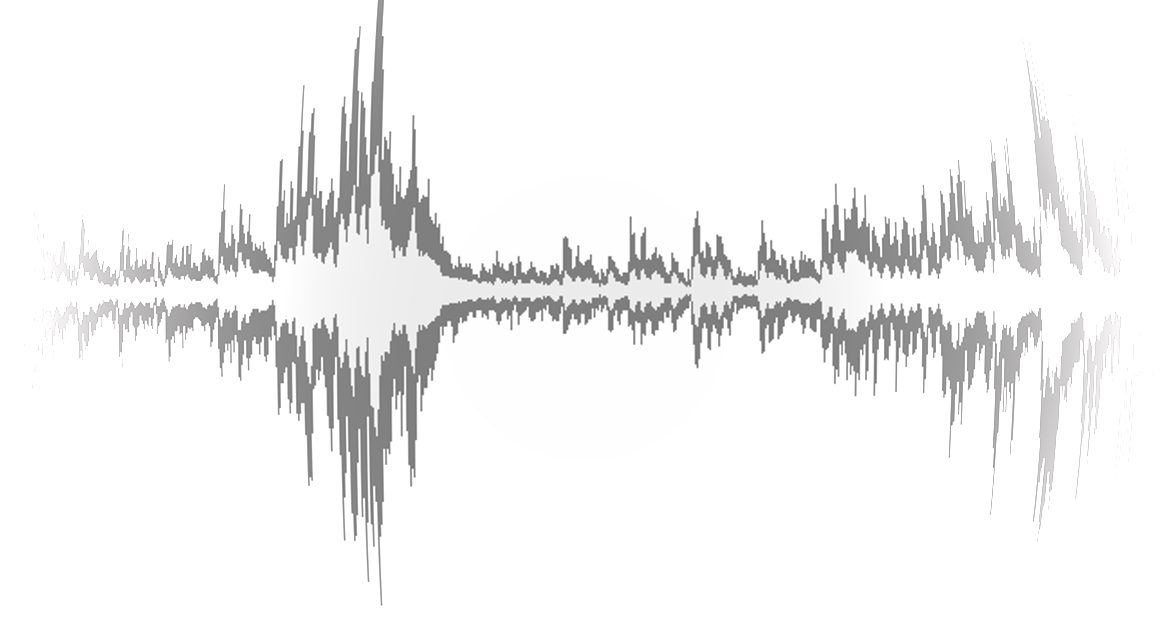
\includegraphics[width=\textwidth,height=3cm]{title}}


\begin{frame}
    \titlepage
    %\vspace{-5mm}
    \begin{flushright}
        \href{http://www.gtcmt.gatech.edu}{
\includegraphics[height=.8cm,keepaspectratio]{../shared/Logo_GTCMT_black}}
    \end{flushright}
\end{frame}


\section[intro]{introduction}
    \begin{frame}\frametitle{sampling and quantization}\framesubtitle{introduction}
        digital signals can only be represented with a limited number of values
        \pause
        
        $\Rightarrow$
        \begin{itemize}
            \item	time discretization:\\ \textbf{sampling}
            \bigskip
            \item	amplitude discretization:\\ \textcolor{gtgold}{\textbf{quantization}}
        \end{itemize}
    \end{frame}
	\begin{frame}\frametitle{sampling and quantization}\framesubtitle{quantization introduction}
		\vspace{-3mm}
        \textbf{quantizer}: \linebreak
		continuous $\mapsto$ discrete (pre-defined set of allowed values)
        
        \figwithmatlab{QuantizedAudio}
    \end{frame}
\section{overview}
	\begin{frame}\frametitle{sampling and quantization}\framesubtitle{quantization: characteristic curve}
        \begin{columns}
            \column{.4\linewidth}
                quantizer \textbf{characteristic curve}:
                \begin{itemize}
                    \item plots output amplitude over input amplitude
                    \smallskip
                    \item   given even number of quantization steps, characteristic curve can be either
                        \begin{itemize}
                            \item   symmetric, or
                            \item   include $0$
                        \end{itemize}
                \end{itemize}
            \column{.6\linewidth}
                \figwithmatlab{QuantizationCharacteristicCurve}
        \end{columns}
    \end{frame}
	\begin{frame}\frametitle{sampling and quantization}\framesubtitle{basic quantization properties}
        \begin{block}{quantization fundamentals}
        \begin{itemize}
            \item   quantization is \textbf{non-linear}:\\ signal is distorted
            \smallskip
            \item   quantization is \textbf{irreversible}:\\ signal cannot be perfectly restored
        \end{itemize}
        \end{block}
	\end{frame}
	
\section[wordlength]{wordlength}
	\begin{frame}\frametitle{sampling and quantization}\framesubtitle{quantization: word length \& number of steps}
		%\vspace{-4mm}
        \only<1>{
		\begin{figure}
			\centering
				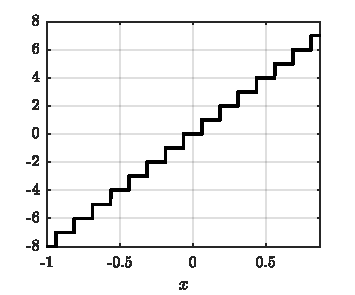
\includegraphics[scale=.7]{QuantizationCharacteristicCurve2-01}
		\end{figure}
        }
		\question{Given a number of quantization steps $\mathcal{M} = 16$ what is the required word length (bits)}
        \bigskip
        $\Rightarrow w = \log_2(16) = \unit[4]{bit}$
		\only<2->{
        \begin{columns}
        \column{.4\linewidth}
        \begin{eqnarray*}
            w &=&\log_2(\mathcal{M})\\
            \mathcal{M} &=& 2^w
        \end{eqnarray*}
        \column{.6\linewidth}
        \begin{figure}
			\centering
				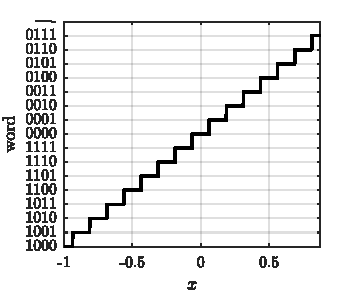
\includegraphics[scale=.7]{QuantizationCharacteristicCurve2-02}
		\end{figure}
        \end{columns}
        }
	\end{frame}
	
	\begin{frame}\frametitle{sampling and quantization}\framesubtitle{quantization: word length examples}
		\begin{table}
			\centering
			\begin{tabular}{llr}
			\hline
				$w$ & $\mathcal{M} = 2^w$ \\
			\hline
				1	&	2\\
				2	&	4\\
				4	&	16\\
				8	&	256\\
				12	&	4096\\
				16	&	65536\\
				20	&	1048576\\
				24	&	16777216\\
			\end{tabular}  
		\end{table}
	\end{frame}
	
	\begin{frame}\frametitle{sampling and quantization}\framesubtitle{scaling, ranges, and words}
        \begin{columns}
        \column{.4\linewidth}
        values are encoded and interpretation is up to the user:
        \begin{itemize}
            \item   word can be translated to integer $\Rightarrow [-8...7]$
            \item   word can be scaled to range of $[-1...1-1/2^{\mathcal{M}-1}]$
                \begin{itemize}
                    \item   standard for floating point systems
                    \item   -1/1 means full scale
                    \item   internal representation independent of quantization word length
                \end{itemize}
        \end{itemize}
        \column{.6\linewidth}
        \figwithmatlab{QuantNumbers}
        \end{columns}
	\end{frame}

\section[error]{quantization error}
	\begin{frame}\frametitle{sampling and quantization}\framesubtitle{quantization error: definition}
		\begin{figure}
			\centering
			 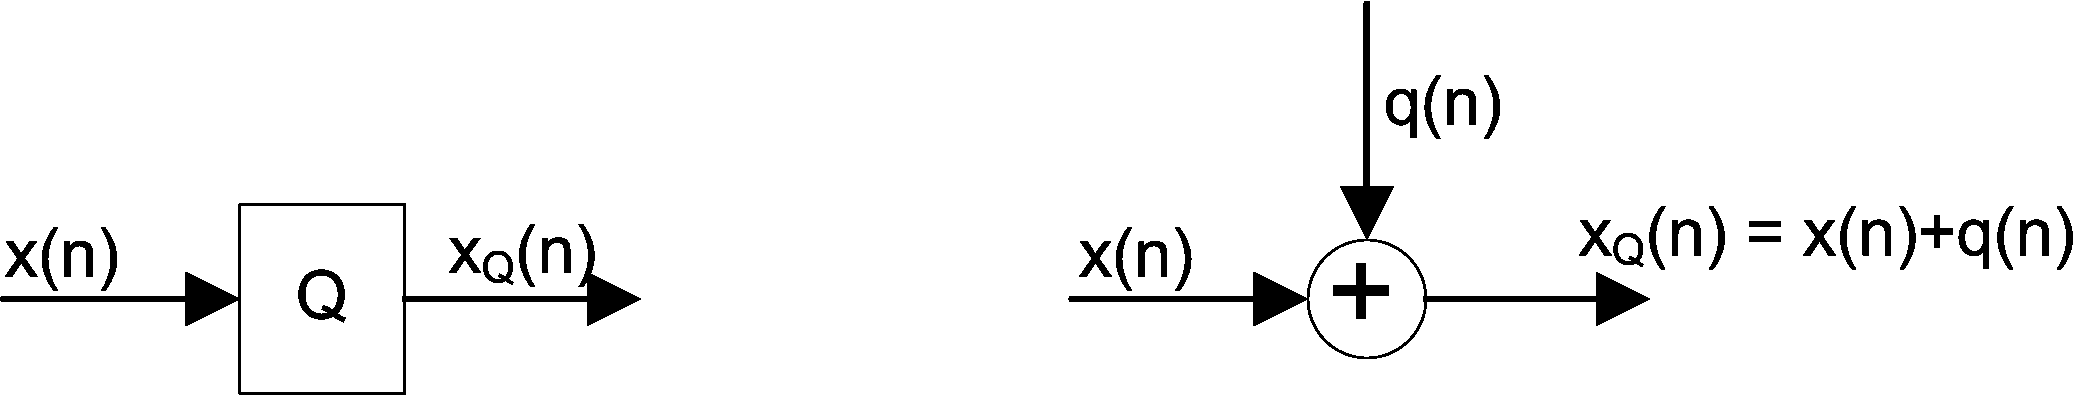
\includegraphics[scale=0.13]{Graph/Flowchart_Quantization}
		\end{figure}
		\begin{equation*}
			q(i) = x_{\mathrm{Q}}(i) - x(i)
		\end{equation*}
	\end{frame}		
	\begin{frame}\frametitle{sampling and quantization}\framesubtitle{quantization error: max.\ amplitude}
		\question{What is the maximum amplitude of the quantization error}
        \begin{columns}
        \column{.2\linewidth}
        \only<3->{
		\begin{equation*}
			|q(i)| \leq \frac{\Delta}{2}
		\end{equation*}
        }
        \column{.8\linewidth}
        \figwithmatlab{QuantizationError}
        \end{columns}
	\end{frame}		

	\begin{frame}\frametitle{sampling and quantization}\framesubtitle{quantization error: pdf 1/2}
		\question{What is the pdf of the quantization error}
        \vspace{-2mm}assuming $\Delta \ll max(|x(i)|)$
        \only<2>{
    	\vspace{-3mm}\begin{figure}[!hbt]
			\begin{center}
			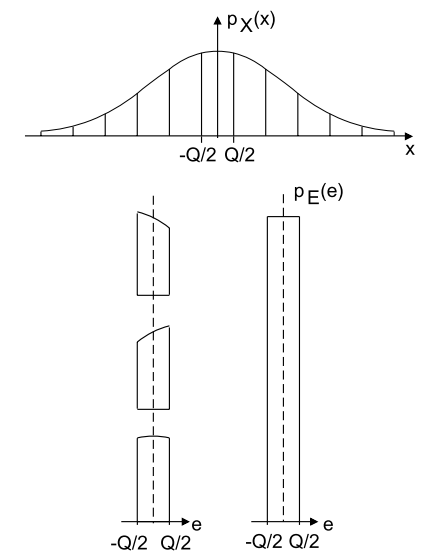
\includegraphics[scale=0.4]{Graph/quantpdf}
			\end{center}
		\end{figure}
        }
        \only<3>{
    	\begin{figure}[!hbt]
			\begin{center}
			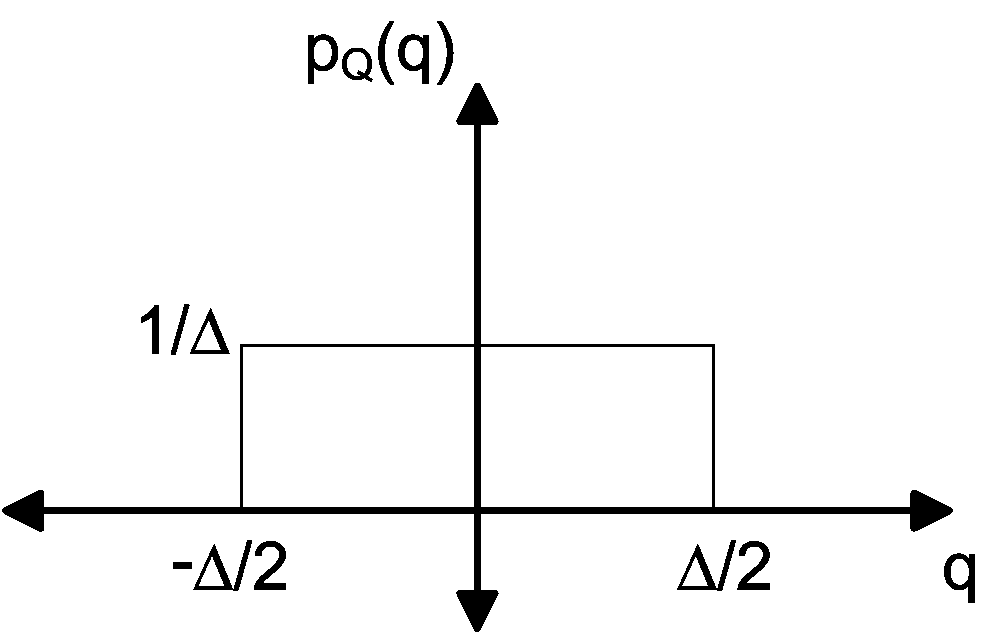
\includegraphics[scale=0.15]{Graph/QuantError_ADV}
			\end{center}
		\end{figure}
        }
	\end{frame}		
	\begin{frame}\frametitle{sampling and quantization}\framesubtitle{quantization error: pdf 2/2}
        \vspace{-3mm}
        it can be shown that the pdf of the quantization error depends (without derivation)
        \begin{itemize}
            \item on the \textbf{variance of the input} signal in relation to the step size
            \item   on the \textbf{pdf of the input} signal
            \smallskip
            \item<2->[$\rightarrow$]   will be \textbf{uniform (and white) for large values of} $\frac{\sigma_X}{\Delta}$
        \end{itemize}
    	\only<2->{
        \begin{figure}
			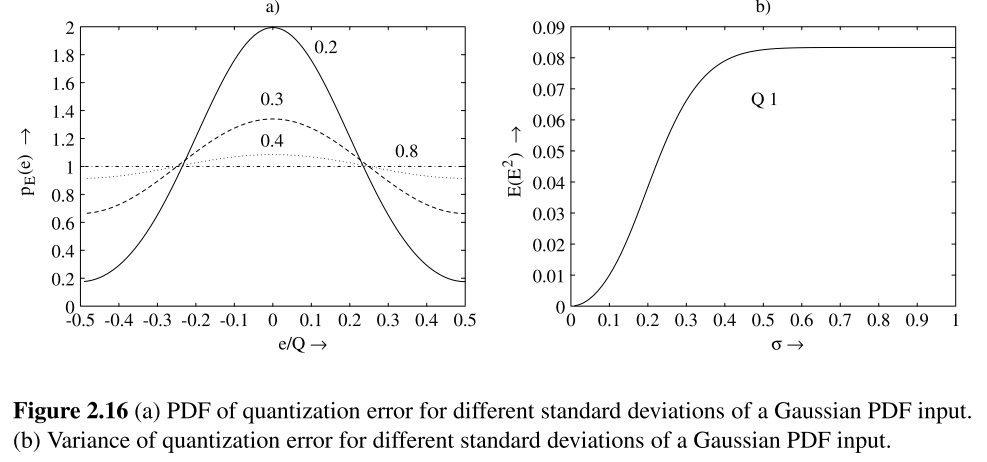
\includegraphics[scale=0.4]{Graph/pdfquanterr_variance}
		\end{figure}
        }
	\end{frame}
	\begin{frame}\frametitle{sampling and quantization}\framesubtitle{quantization error: power}
        \vspace{-2mm}
        \question{how to compute the power $W_\mathrm{Q}$ of the quantization error}
        \vspace{-2mm}
        \begin{footnotesize}
        from PDF:
        \begin{eqnarray*}
            W_\mathrm{Q} &=& \int\limits_{-\nicefrac{\Delta}{2}}^{\nicefrac{\Delta}{2}}{q^2\cdot \underbrace{p_\mathrm{Q}(q)}_{\nicefrac{1}{\Delta}}}\, dq\\
            \pause
            &=& \frac{1}{\Delta}\int\limits_{-\nicefrac{\Delta}{2}}^{\nicefrac{\Delta}{2}} q^2\, dq\\
            \pause
            &=& \frac{1}{\Delta} \left[\frac{1}{3}q^3\right]_{-\nicefrac{\Delta}{2}}^{\nicefrac{\Delta}{2}}\\
            \pause
            &=& \frac{1}{3\Delta}\left(\frac{\Delta^3}{8} + \frac{\Delta^3}{8}\right)\\
            \pause
            &=& \frac{\Delta^2}{12}
        \end{eqnarray*}
        \end{footnotesize}
        
	\end{frame}
	\begin{frame}\frametitle{sampling and quantization}\framesubtitle{quantization error: spectrum}
        quantization error of a full-scale sinusoidal (2,4,8,12 bits)
        \figwithmatlab{QuantizationErrorSpectrum}
	\end{frame}		
\section[audio]{audio examples}
	\begin{frame}\frametitle{sampling and quantization}\framesubtitle{quantization: audio examples}
        \begin{footnotesize}
		\begin{table}
			\begin{center}
				\begin{tabular}{lcccccc}
                $w$ & $x_\mathrm{Q,sine}(i)$ & $q_\mathrm{sine}(i)$ & $x_\mathrm{Q,speech}(i)$ & $q_\mathrm{speech}(i)$ & $x_\mathrm{Q,music}(i)$ & $q_\mathrm{music}(i)$\\\hline
                $16$& \includeaudio{sine_quant_16bit} & \includeaudio{sine_quant_16bit_Q}  &
                     \includeaudio{sqam_49_female_16bit} & \includeaudio{sqam_49_female_16bit_Q} &
                     \includeaudio{bigband_16bit} & \includeaudio{bigband_16bit_Q} \\

                $12$ &\includeaudio{sine_quant_12bit} & \includeaudio{sine_quant_12bit_Q}  &
                     \includeaudio{sqam_49_female_12bit} & \includeaudio{sqam_49_female_12bit_Q} &
                     \includeaudio{bigband_12bit} & \includeaudio{bigband_12bit_Q} \\
                $8$ &\includeaudio{sine_quant_8bit} & \includeaudio{sine_quant_8bit_Q}  &
                     \includeaudio{sqam_49_female_8bit} & \includeaudio{sqam_49_female_8bit_Q} &
                     \includeaudio{bigband_8bit} & \includeaudio{bigband_8bit_Q} \\
                $6$ &\includeaudio{sine_quant_6bit} & \includeaudio{sine_quant_6bit_Q}  &
                     \includeaudio{sqam_49_female_6bit} & \includeaudio{sqam_49_female_6bit_Q} &
                     \includeaudio{bigband_6bit} & \includeaudio{bigband_6bit_Q} \\
                $4$ &\includeaudio{sine_quant_4bit} & \includeaudio{sine_quant_4bit_Q}  &
                     \includeaudio{sqam_49_female_4bit} & \includeaudio{sqam_49_female_4bit_Q} &
                     \includeaudio{bigband_4bit} & \includeaudio{bigband_4bit_Q} \\
                $2$ &\includeaudio{sine_quant_2bit} & \includeaudio{sine_quant_2bit_Q}  &
                     \includeaudio{sqam_49_female_2bit} & \includeaudio{sqam_49_female_2bit_Q} &
                     \includeaudio{bigband_2bit} & \includeaudio{bigband_2bit_Q} 
				\end{tabular}  
			\end{center}
		\end{table}
        \end{footnotesize}
    \end{frame}		
	
\section[SNR]{SNR}
	\begin{frame}\frametitle{sampling and quantization}\framesubtitle{quality assessment of a quantizer: SNR}
        Signal-to-Noise Ratio (SNR): 
        \begin{itemize}
            \item power of the signal in relation to power of the (quantization) noise
                \begin{equation*}\nonumber
                    SNR' = \frac{\text{signal energy}}{\text{noise energy}} = \frac{W_{\mathrm{S}}}{W_{\mathrm{Q}}}
                \end{equation*}
            \smallskip
            \item<2-> often in decibel
                \begin{equation*}\label{eq:snr}
                    SNR = 10\cdot\log_{10}\left(\frac{W_{\mathrm{S}}}{W_{\mathrm{Q}}}\right)\; [dB] 
                \end{equation*}
            \smallskip
            \item<3-> SNR grows by
                \begin{itemize}
                    \item   reducing the noise power
                    \item   increasing the signal power
                \end{itemize}
        \end{itemize}
	\end{frame}		
	
	\begin{frame}\frametitle{sampling and quantization}\framesubtitle{quantization: SNR 1/3}
		\question{What is the SNR of a quantized full-scale sinusoidal}
        \begin{footnotesize}
			\begin{equation*}\nonumber
				SNR = 10\cdot\log_{10}\left(\frac{W_{\mathrm{S}}}{W_{\mathrm{Q}}}\right)\; [dB] 
			\end{equation*}
			
			\hspace{3mm}use: $sin^2(t) = \frac{1-cos(2t)}{2}$
			\pause
		\begin{eqnarray*}
			W_\mathrm{S} &=& \frac{A^2}{2}\; \stackrel{\rightarrow}{\text{\tiny{full-scale}}} W_\mathrm{S} =\frac{(\Delta\cdot 2^{w-1})^2}{2}\\
			W_\mathrm{Q} &=& \frac{\Delta^2}{12}\\
			\pause
			\frac{W_\mathrm{S}}{W_\mathrm{Q}} &=& \frac{3}{2}\cdot 2^{2w}
		\end{eqnarray*}
        \pause
			\begin{equation*}\nonumber
				SNR = w\cdot 20\log_{10}\left(2\right) + 10\cdot\log_{10}\left(\frac{3}{2}\right)\; [dB] 
			\end{equation*}
        \end{footnotesize}
    \end{frame}		
	\begin{frame}\frametitle{sampling and quantization}\framesubtitle{quantization: SNR 2/3}
        \question{derive the SNR for a full-scale square wave}
        \begin{footnotesize}
			\begin{equation*}\nonumber
				SNR = 10\cdot\log_{10}\left(\frac{W_{\mathrm{S}}}{W_{\mathrm{Q}}}\right)\; [dB] 
			\end{equation*}
			
		\begin{eqnarray*}
			W_\mathrm{S} &=& {A^2}\; \stackrel{\rightarrow}{\text{\tiny{full-scale}}} W_\mathrm{S} ={(\Delta\cdot 2^{w-1})^2}\\
			W_\mathrm{Q} &=& \frac{\Delta^2}{12}\\
			\pause
			\frac{W_\mathrm{S}}{W_\mathrm{Q}} &=& {3}\cdot 2^{2w}
		\end{eqnarray*}
        \pause
			\begin{equation*}\nonumber
				SNR = w\cdot 20\log_{10}\left(2\right) + 10\cdot\log_{10}\left(3\right)\; [dB] 
			\end{equation*}
        \end{footnotesize}
	\end{frame}		
	\begin{frame}\frametitle{sampling and quantization}\framesubtitle{quantization: SNR 3/3}
		\vspace{-5mm}\toremember{}
        %\vspace{-3mm}
        \begin{block}{Signal-to-Noise Ratio}
			\centering
			\begin{equation*}
				SNR = 6.02\cdot w + c_{\mathrm{S}}\quad [dB]
			\end{equation*}
            \vspace{-2mm}
			\begin{itemize}
				\item	every additional bit adds app.\ \unit[6]{dB} SNR
				\item	constant $c_{\mathrm{S}}$ depends on signal (scaling and PDF shape)
			\end{itemize}
		\end{block}
        \pause
		\begin{itemize}
            \item[] SNR for different input signal examples
                \begin{itemize}
                    \item	square wave (full scale): $c_{\mathrm{S}} =  \unit[4.77]{dB}$
                    \item	sinusoidal wave (full scale): $c_{\mathrm{S}} =  \unit[1.76]{dB}$
                    \item	rectangular {PDF} (full scale): $c_{\mathrm{S}} =  \unit[0]{dB}$
                    \item	Gaussian {PDF} (full scale = $4\sigma_{g}$): $c_{\mathrm{S}} =  \unit[-7.27]{dB}$
                \end{itemize}
		\end{itemize}
	\end{frame}		
	\begin{frame}\frametitle{sampling and quantization}\framesubtitle{quantization: word length and SNR}
			\begin{table}
			\centering
				\begin{footnotesize}
					\begin{tabular}{lccc}
					\hline
						\textbf{w} & \textbf{$\Delta$} & \textbf{Max.\ Amp} & \textbf{theo.\ SNR} \\
					\hline
						8 (Int)	&	$\pm1$ & $0\ldots255$ & $\approx$\unit[48]{dB}\\
						16 (Int)	&	$\pm1$ & $-32768\ldots32767$ & $\approx$\unit[96]{dB}\\
						20 (Int)	&	$\pm1$ & $-524288\ldots524287$ & $\approx$\unit[120]{dB}\\
						24 (Int)	&	$\pm1$ & $-16777216\ldots16777215$ & $\approx$\unit[144]{dB}\\
					\hline
						32 (Float)	&	$\pm1.175\cdot10^{-38}$ & $\pm3.403\cdot10^{1038}$ & \unit[1529]{dB}\\
						64 (Float)	&	$\pm2.225\cdot10^{-308}$ & $\pm1.798\cdot10^{10308}$ & \unit[12318]{dB}\\
					\hline
					\end{tabular}  
				\end{footnotesize}
			\end{table}
            \bigskip
	\end{frame}	
	
	\begin{frame}\frametitle{sampling and quantization}\framesubtitle{quantization: SNR and auditory sensation area}
        \question{so how many bits do we need}
	    \only<2>{
        \begin{figure}
			\centering
				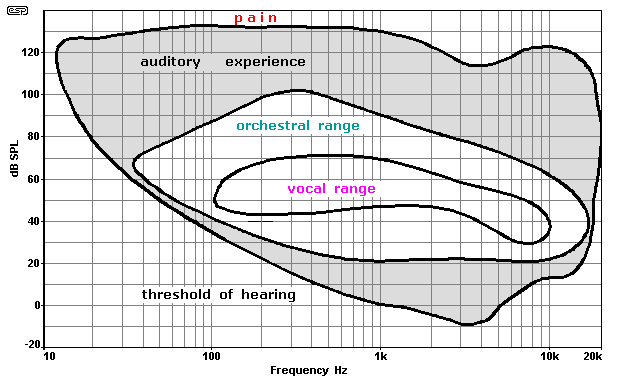
\includegraphics[scale=0.5]{Graph/hoerfeld}
		\end{figure}
        }
	    \only<3->{
        \vspace{-3mm}
        \begin{figure}
			\centering
				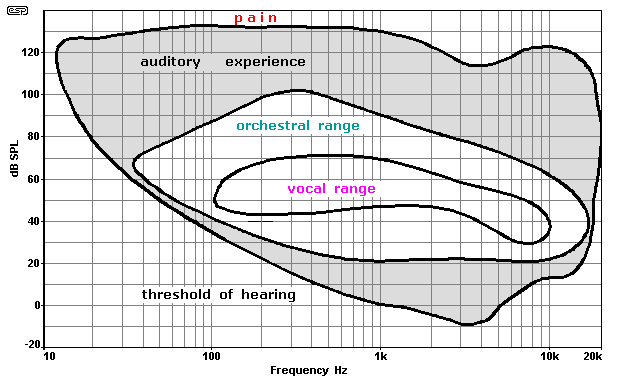
\includegraphics[scale=0.25]{Graph/hoerfeld}
		\end{figure}
        }
        \begin{itemize}
            \item<3->   to cover the whole range of hearing: 20--24 bit
            \item<3->   practically, a lower range is sufficient as the dynamic range of recordings has to be much lower
            \item<3->   in production with many processing and possible requantization steps, high resolution (if possible floating point) is recommended
        \end{itemize}
	\end{frame}

\section[clipping]{clipping}

	\begin{frame}\frametitle{sampling and quantization}\framesubtitle{quantization: clipping}
        \begin{columns}
        \column{.7\linewidth}
	    \vspace{-5mm}
            \figwithmatlab{Clipping}
        \column{.3\linewidth}
            
            \bigskip
            \includeaudio{sine}
            \bigskip
            \bigskip
            \smallskip
             
            \includeaudio{sine_clipped}
            \bigskip
            \bigskip
            \smallskip
            
            \includeaudio{sine_wrapped}
        \end{columns}
	\end{frame}	
	
	\begin{frame}\frametitle{sampling and quantization}\framesubtitle{quantization: clipping and SNR}
	    \figwithmatlab{Snr}
        
     \begin{itemize}
         \item[] full scale:
            \begin{itemize}
                \item   absolute maximum before clipping
                \item   usually $1$ (in floating point systems)
                \item   marks \unit[0]{dbFS}
            \end{itemize}
     \end{itemize}
	\end{frame}
	

	\section{summary}	
		\begin{frame}{sampling and quantization}{quantization: summary }
			\vspace{-3mm}
            \begin{itemize}
                \item   quantization is  \textbf{non-linear} \& \textbf{irreversible}
                    \begin{itemize}
                        \item   information is lost
                        \item   error is introduced
                    \end{itemize}
                \smallskip
                \item<2->   quantization \textbf{error}
                    \begin{itemize}
                        \item   power is determined by number of bits (wordlength)
                        \item   is approximately white noise (flat spectrum and uncorrelated to signal) when the signal power is much higher than the quantization step size
                        \item   special severe case: clipping
                    \end{itemize}
                \smallskip
                \item<3->   \textbf{SNR} is used to assess quantizer quality
                    \begin{itemize}
                        \item   depends on both signal power and quant error power (ratio)
                        \item   each additional bit gains \unit[6]{dB} SNR
                        \item   different signals with identical maximum amplitude yield different SNRs
                    \end{itemize}
                \smallskip
                \item<4-> \textbf{typical word lengths} include
                    \begin{itemize}
                        \item   \unit[8]{bit}: phone
                        \item   \unit[16]{bit}: consumer audio
                        \item   \unit[24]{bit} and higher: production audio
                    \end{itemize}
			\end{itemize}
		\end{frame}
 

\end{document}

